\documentclass[sigconf]{acmart}

% just in case
\usepackage{etex}

% does not seem to work with sigconf template
%\usepackage{cite}

\usepackage{tikz}
	\usepackage{pgf, pgfplots, pgfplotstable}
	\usetikzlibrary{arrows,automata}
	\usetikzlibrary{patterns}

\usepackage[utf8]{inputenc}
\usepackage[T1]{fontenc}
\usepackage{hyperref}
\usepackage{blindtext}
\usepackage{booktabs}
\usepackage{paralist}
\usepackage{listings,multicol}
\usepackage{lipsum}

\usepackage{enumerate}
\usepackage{subcaption}
\usepackage{cleveref}
\usepackage{ucs}
\usepackage{framed}

\setlength\parindent{0pt}

\renewcommand{\sf}[1]{\textsf{#1}}
\renewcommand{\tt}[1]{\texttt{#1}}

\usepackage[zerostyle=d]{newtxtt}
\usepackage[T1]{fontenc}

%\usepackage[labelfont=bf]{caption}

\definecolor{lightgrey}{HTML}{FFFFFF}

\hypersetup{
    colorlinks,
    linkcolor={red!65!black},
    citecolor={blue!50!black},
    urlcolor={blue!80!black}
}

\usepackage{listings}  

\lstset{
	language=PHP,
	extendedchars = \true,
	basicstyle=\ttfamily\footnotesize,
	basewidth={0.5em,0.4em}, % for other columns settings
	commentstyle = \color{black},
	columns=fullflexible,
	numbers=left,
	numberstyle=\tiny,
	frame=tb,
	showstringspaces=false,
	xleftmargin=2em,
	framexleftmargin=1.5em,
	backgroundcolor=\color{lightgrey},
	inputencoding = utf8x,
    keepspaces = true,
    keywordstyle = \bfseries
}

%\newcommand{\dollar}{\mbox{\textdollar}}


\newcommand*{\origrightarrow}{}
\let\oldarrow\textrightarrow
\renewcommand*{\textrightarrow}{\fontfamily{cmr}\selectfont\origrightarrow}

% ARIAL
%\usepackage{helvet}
%\renewcommand{\familydefault}{\sfdefault}


% TIMES
%\usepackage{mathptmx}% http://ctan.org/pkg/mathptmx



\usepackage{xcolor}

% Copyright
%\setcopyright{none}
%\setcopyright{acmcopyright}
%\setcopyright{acmlicensed}
\setcopyright{rightsretained}
%\setcopyright{usgov}
%\setcopyright{usgovmixed}
%\setcopyright{cagov}
%\setcopyright{cagovmixed}


% DOI
%\acmDOI{10.475/123_4}

% ISBN
%\acmISBN{123-4567-24-567/08/06}

%Conference
\acmConference[ISSTA'17]{ACM Woodstock conference}{July 2017}{Santa Barbara,
 California, USA}
%\acmYear{1997}
%\copyrightyear{2016}

%\acmPrice{15.00}


\begin{document}
\title{Does It Scale? Symbolic Execution of PHP Web Applications}
%\titlenote{Produces the permission block, and copyright information}
\subtitle{Output-oriented Symbolic Execution for Static Output Approximation}
%\subtitlenote{The full version of the author's guide is available as  \texttt{acmart.pdf} document}


%\author{Stefan Mühlbauer}
\affiliation{%
  %\institution{Technische Universität Braunschweig}
  %\streetaddress{P.O. Box 1212}
  %\city{Braunschweig} 
  %\state{Germany} 
  %\postcode{43017-6221}
}
%\email{s.muehlbauer@tu-bs.de}

%\author{Christian Kästner}
%\orcid{1234-5678-9012}
\affiliation{%
  %\institution{Carnegie Mellon University}
  %\streetaddress{5000 Forbes Avenue}
  %\city{Pittsburgh} 
  %\state{PA} 
  %\postcode{15217}
}
%\email{s.muehlbauer@tu-bs.de}

%\author{Tien N. Nguyen}
%\orcid{1234-5678-9012}
\affiliation{%
  %\institution{University of Texas at Dallas}
  %\streetaddress{P.O. Box 1212}
  %\city{Braunschweig} 
  %\state{Germany} 
  %\postcode{43017-6221}
}
%\email{s.muehlbauer@tu-bs.de}


% The default list of authors is too long for headers}
\renewcommand{\shortauthors}{
	%\textcolor{blue}{put shortauthors here}
}


\begin{abstract}
Dynamic web applications have become widely popular and are to a large portion
based on the scripting language PHP. Dynamic languages like PHP challenge
static analysis, as they generate code at runtime. One approach to unfold their
staged nature is symbolic execution by approximating client page output.
Knowledge about possible output enables a range of developer tools and analyses
for vulnerability detection.

However, previous tools have only been evaluated for smaller systems and
scalability for larger systems has not been shown. We criticize the missing
evalaution of practicality of respective tools and ask whether symbolic
execution for output approximation for PHP is scalable and what limitations can
be faced. This paper presents our experiences with re-implementing and
extending a previous symbolic execution engine for PHP that we evaluate for
several large PHP systems.
We find that dynamic language features are likely to be resolved imprecisely
for symbolic values and impede symbolic execution. We explore
strategies to mitigate limitations based on previous work on dynamic symbolic
execution by manually providing concrete rather than symbolic values.
\end{abstract}

%
% The code below should be generated by the tool at
% http://dl.acm.org/ccs.cfm
% Please copy and paste the code instead of the example below. 
%
\begin{CCSXML}
<ccs2012>
 <concept>
  <concept_id>10010520.10010553.10010562</concept_id>
  <concept_desc>Computer systems organization~Embedded systems</concept_desc>
  <concept_significance>500</concept_significance>
 </concept>
 <concept>
  <concept_id>10010520.10010575.10010755</concept_id>
  <concept_desc>Computer systems organization~Redundancy</concept_desc>
  <concept_significance>300</concept_significance>
 </concept>
 <concept>
  <concept_id>10010520.10010553.10010554</concept_id>
  <concept_desc>Computer systems organization~Robotics</concept_desc>
  <concept_significance>100</concept_significance>
 </concept>
 <concept>
  <concept_id>10003033.10003083.10003095</concept_id>
  <concept_desc>Networks~Network reliability</concept_desc>
  <concept_significance>100</concept_significance>
 </concept>
</ccs2012>  
\end{CCSXML}

\ccsdesc[500]{Computer systems organization~Embedded systems}
\ccsdesc[300]{Computer systems organization~Redundancy}
\ccsdesc{Computer systems organization~Robotics}
\ccsdesc[100]{Networks~Network reliability}

% We no longer use \terms command
%\terms{Theory}

\keywords{ACM proceedings, \LaTeX, text tagging}

\maketitle

\section{Introduction}
With the emerging world wide web, dynamic web applications have become
widely popular. Various different implementation techniques have emerged,
ranging from technologies for programming languages (JSP, ASP .NET) and web
application frameworks for  script languages (Ruby On Rails, Django) to
languages tailored specifically to the domain of web applications. PHP
\cite{phpNET} is a programming language focused on server-side application
development. As of 2012, it was used by 78.8 percent of the ten million most popular websites (according
to Alexa popularity ranking) \cite{alexaPHP}, ranking 7th on the TIOBE
programming community index \cite{tiobePHP}, and was the ranked as the 6th
most popular language on GitHub \cite{githubPHP}.

A common characteristic of all dynamic web applications is their
\emph{staged nature}: A dynamic web application as a whole
consists of both static code, such as scripts, and dynamically generated code,
such as client page output. The latter code, although assembled at
runtime, may contain client-side parts of the web application, such as
JavaScript. So, to study dynamic web applications in its entirety, we need to
consider both static as well as dynamic aspects of systems.

\emph{Symbolic execution} is a static analysis technique between program testing
and program proving. For a program, symbolic values are
used instead of concrete inputs \cite{Darringer1978,King1976}. The underlying
concept is to map program input to program output: Symbolic values are used and
propagated throughout the symbolic execution and keep dependencies for program
output traceable. This analysis technique helps unfold the \emph{staged} nature
of dynamic web applications. Since every feasible path can be executed the
symbolic output contains both invariant output as well as output variants that
depend on program input.

Knowledge about different output variants is leveraged by a number of
analyses for the domain of web applications. Previous work presented tools
for detecting and locating HTML validation errors
\cite{Nguyen:2011:AFH:2190078.2190142}, computing program slices across
server-side and client-page code \cite{Nguyen:2015:CPS:2786805.2786872}, or
easing development and maintenance by extending IDE support for web applications
with code navigation \cite{Nguyen:2015:VIS:2819009.2819140,Nguyen:2014:BCG:2635868.2635928}.
Moreover, knowledge of output variants can increases code coverage for
output-oriented testing \cite{Alshahwan2011}.

Despite the various use cases for analyses based on an approximated output
model, static output approximation for PHP web applications using symbolic
execution has so far only been evaluated for small systems that are not
maintained anymore. The tools presented by previous work
\cite{Nguyen:2015:VIS:2819009.2819140,Nguyen:2014:BCG:2635868.2635928,Nguyen:2015:CPS:2786805.2786872,Nguyen:2011:AFH:2190078.2190142}
though are only practical, if for a given system the symbolic execution engine
is scalable, i.e., will also approximate output accurately for larger and more
recent systems with acceptable time and space consumption.

To investigate the question, whether we can have a practical and scalable
symbolic executoin engine, we re-implemented the engine with the specifications
of the previous symbolic execution semantics \cite{Nguyen:2014:BCG:2635868.2635928} for PHP and additional features, such
as object-oriented programming. We evaluate our
symbolic execution engine for several large-scale and modern PHP systems.

During the introduction of new semantics, we addressed two  trade-offs between
accuracy of our execution and performance: For method calls with ambiguous
targets as well as concrete execution of loops the number of program states can
become infeasible. This may require additional engineering adjustments to tame
the state space explosion at cost of accuracy.

Based on observations we identify conceptual limitations of symbolic
execution for PHP.  Dynamic features such as indirect function invocations and
include expression require concrete information to be evaluated properly. Since
these expressions may be assembled at runtime and can contain symbolic
information, for many cases this restricts a symbolic execution engine from
further execution.
Although some effort to statically approximate include expression can be spent,
it is often non-trivial since expressions can contain information coming from
various inputs including databases, user inputs or configuration files. We
empirically evaluate our observations for a corpus including large, actively maintained PHP systems.

Our key contribution in this paper include (1)  a new tool infrastructure to
statically approximate the client-page output for PHP web applications using
symbolic execution and (2) a report of observations for state-of-the-art
web applications as well as an empirical evaluation of conceptual limitations
of symbolic executions for PHP web applications.

\section{State Of the Art}\label{sec:stateoftheart}
This section recaps the idea of symbolic
execution, the tools which make use of it, and both conceptual and
language-related limitations.

\subsection{Symbolic Execution}
Symbolic execution is a static analysis technique that was proposed by King
\cite{King1976} in 1976. Symbolic execution allows to explore feasible paths in a program. Based on normal program execution, the execution semantics
is extended to handle symbolic values. An execution becomes symbolic by
assuming symbolic values as program inputs rather than obtaining concrete
values \cite{King1976,Darringer1978}. These symbolic values are then propagated
and used throughout the execution. 

Execution starts with a tautology path
condition. The control-flow can be split whenever the decision between branches
is ambiguous. This is the case, when conditional expressions, for example for
if-statements, evaluate to a symbolic value rather than an actual result.
The corresponding path conditions (guards for instance) are conjoined with the
previous path condition \cite{King1976}. Additionally, the conjoined path
condition can be checked for satisfiability in order to exclude infeasible
paths. 


\subsection{Static Output Approximation for PHP} \label{sec:workflow}
Symbolic execution is not dedicated to a particular
programming language. For dynamic web applications, in our case for web
applications written in PHP, it can be used to approximate all possible client
page output variants. Before we present in detail existing tools that aim to
ease development and maintenance of PHP web applications, we illustrate how output
approximation using symbolic execution is pursued by starting with a small
example.

\begin{figure}[t]
	\centering
	\begin{subfigure}[center]{0.48\textwidth}%%[multicols=1]
\begin{lstlisting}
<form method="POST">
  <input type="text" name="name">
  <input type="submit" value="Submit">
</form>

<?php
function make_titles($arg, $n) {
  $is = shuffle(array(1,2,3));
  while ($n < $is[0]) {
    echo "<h1>" . $arg . "</h1><br />";
    $n = $n + 1;
  }
}
  
call_user_func("make_titles", "Headline", 4);

$greeting = "Hello " . $_POST['name'] .  "!";
if (!isset($_POST['name'])) {
  echo "No name entered!";
} else {
  echo $greeting;
}
?>
\end{lstlisting}
		\caption{Snippet of server-side HTML and PHP web application code.
		\label{fig:web_application}}
    \end{subfigure}

	\vspace{2mm}    
    
    ~ %add desired spacing between images, e. g. ~, \quad, \qquad, \hfill etc. 
      %(or a blank line to force the subfigure onto a new line)
    \begin{subfigure}[center]{0.48\textwidth}
\begin{lstlisting}[mathescape]
<form method="POST">
  <input type="text" name="name">
  <input type="submit" value="Submit">
</form>

// #repeat n < shuffle(is)
<h1>Headline</h1><br />
// #endrepeat

// #if !isset(name)
No name entered!
// #else
Entered $\alpha$!
// #endif

\end{lstlisting}
		\caption{
			Approximated client page output of the server-side code in Figure
			\ref{fig:web_application}. The directives in lines 6 and 8 highlight output
			that can be repeated an arbitrary number of times, the directives in line 10
			and 14 mark two alternative output parts.
			\label{fig:output_example}
		}
    \end{subfigure}
    \vspace{2mm}
    \caption{
    	Illustration of static ouptut approximation using symbolic
    	execution
    	\label{fig:code_example}
    }
\end{figure}

Figure \ref{fig:code_example} shows two code listings. The snippet of server-side web
application code in Figure \ref{fig:web_application} contains both HTML code
(input form in lines 1 -- 4) as well as PHP code: First, the function
\texttt{make\_titles} defined in lines 7 – 13 prints the string \texttt{\$arg} passed as an argument between zero and an arbitrary number of
times. Second, the function is indirectly called using the built-in mechnism
\texttt{call\_user\_func} in line 15 with the string \texttt{Headline} and
\texttt{4} as arguments.  Finally, the input from the form in lines 1 – 4 is
used: The variable \texttt{\$greeting} consists of three concatenated strings,
\texttt{Hello}, the value of input field \texttt{name}, and an exclamation mark.
For the greeting there are two possible client page output
variants: If the input field \texttt{name} is empty at runtime, line 19 is
executed and \texttt{No name entered!} is printed, or, if a name was entered,
line 21 is executed and the greeting constructed in line 17 is printed.

The following symbolic execution semantics for PHP features based on
previous work \cite{Nguyen:2014:BCG:2635868.2635928} illustrate the necessary
modifications and extensions made to handle the level of ambiguity that comes with handling symbolic values. In addition to normal output, the
output approximation contains preprocessor directives to express
repeatable parts as well as output variants. All approximated client page
output corresponding to Figure \ref{fig:web_application} consisting of two different variants
is illustrated in Figure \ref{fig:output_example}.

First, for loops in the previous execution semantics
\cite{Nguyen:2014:BCG:2635868.2635928} only one iteration is executed instead of
an arbitrary number of iterations. Since a loop condition can contain symbolic
values, it might not be feasible to determine whether, and if so, when a loop
execution terminates. Hence, any output constructed during the single loop
iteration is highlighted (\texttt{repeat \ldots endrepeat}) to possibly be
repeated an arbitrary number of times. The output in line 7 is marked to be
repeated an arbitrary number of times, as the number of loop iterations cannot
be determined statically. 

Second, a similar procedure applies to recursive
functions. Once called, a recursive function is  also only executed to recursion
depth one per call, and any subsequent invocation of that function returns a
symbolic value. This, again, is due to the difficulty to determine the exact
recursion depth similar to the number of loop iterations.

Third, any form of user interaction providing input data as well as any form of input referred
to from the deployment context of the web application, i.e. configuration files
or databases, is assumed to be symbolic. The context variable
\texttt{\$\_POST} represents input submitted to the server and, hence, is
symbolic as every program input is per definition substituted by symbolic values. Finally, the
output in lines 11 and 13 respectively are marked as alternative variants
(\texttt{if \ldots else \ldots endif}) as symbolic execution of lines 18 – 22
in Figure \ref{fig:web_application} will explore both different branches.

\subsection{Symbolic-Execution-based Tools For PHP}\label{sec:existing_tools}
All tools proposed so far leverage a representation of all possible HTML client
page output. Since any single client page output variant can be analyzed this
enables tool support addressing the web application as a whole in spite of its
staged nature, where parts of the web application are
generated dynamically.
Based on the approximated output representation, subsequent analyses can be
conducted:
\begin{itemize}
	\item \emph{PhpSync}: Using all variants of  HTML client page output, every
	single one can be statically checked for markup validity, i.e., if the web page
	conforms to syntactical specifications for HTML and other client-side
	languages. After the tool detects validation errors, auto-fixes
	can be provided. Otherwise, it traces validation errors back to
	source code responsible for the defect, which then can be refactored manually
	\cite{Nguyen:2011:AFH:2190078.2190142}. 

	\item \emph{WebSlice}: Program slices enable to extract and understand the
	impact of changes in an application. To consider all of a dynamic web
	application for program slices, client page output needs to be taken into
	account. WebSlice combines PHP data-flow information with an output
	approximation to enable program slices across different languages
	\cite{Nguyen:2015:CPS:2786805.2786872}.

	\item \emph{Varis}: Editor services such as “jump to declaration” are
	nontrivial for dynamic web applications due to their staged nature. Varis
	provides editor services across stages for client-side code: Starting with an
	ouput approximation a callgraph with conditional edges is constructed, which
	allows navigation in client-site code (HTML, JS and CSS) although it is
	embedded in server-side code
	\cite{Nguyen:2015:VIS:2819009.2819140,Nguyen:2014:BCG:2635868.2635928}.

\end{itemize}

\subsection{Assumptions And Limitations}\label{sec:limitations}
In addition to the assumptions introduced by symbolic execution, such as
symbolic inputs and one-time loop execution, the symbolic execution
engine described in previous work \cite{Nguyen:2014:BCG:2635868.2635928} does
not support advanced language features, including object-oriented programming. Moreover, the range of
standard library functions supported are mostly string operations, yet PHP
provides a large collection of functions for array operations.
All three analyses described in Section \ref{sec:existing_tools} though have
only been applied to systems that are small and not maintained any more. Despite the
functional benefits these tools provide to developers, their practicality for
large and modern systems with respect to advanced language support has not been
evaluated.

\section{Scalable Output Approximation?} \label{sec:3}
The main objective of this experience report is to investigate whether we can
build a scalable symbolic execution engine as it is the underlying technique
for static output approximation in previous work
\cite{Nguyen:2011:AFH:2190078.2190142,Nguyen:2014:BCG:2635868.2635928,Nguyen:2015:CPS:2786805.2786872,Nguyen:2015:VIS:2819009.2819140}.
Our vision is a practical symbolic execution, i.e., it computes an accurate
approximation for large and modern PHP systems with reasonable time and space consumption.
We approach this goal by re-implementing the symbolic execution semantics  of
\sf{PhpSync} \cite{Nguyen:2014:BCG:2635868.2635928} and extending it with support for additional language
including object-oriented programming and array operations. We aim to support symbolic
execution for a real-world example system of reasonable size that incorporates
the missing language features described in Section \ref{sec:limitations}.
\textsf{WordPress} is a popular open-source Content Management System (CMS)
with around 300.000 lines of code that provides a vivid
plug-in environment and is used.  The full implementation of \sf{Oak}, the test
suite as well as or test corpus (see Section \ref{sec:experiment_setup}) can be found at
\url{http://www.github.com/smba/oak}.

For our implementation of a symbolic execution engine for PHP, Oak, we have
chosen a test-driven approach with continuous integration using regression
tests based on \sf{WordPress} and \sf{SchoolMate} (see Section
\ref{sec:experiment_setup}). For \sf{SchoolMate}, a rather straightforward and
simple system, which we chose to compare our approximation results to those of
\sf{PhpSync}, we could achieve similar output approximation results. For
\sf{WordPress} though, we did not achieve high code coverage or an accurate
approximation for \sf{WordPress} as we faced a number of obstacles hindering
symbolic execution in different ways.

\subsection{Experience Report}\label{sec:experience_report}
We document our design choices we made, apparent trade-offs we
recognized, and limitations we faced on our way towards a scalable symbolic
execution engine; and what we have learned from bypassing limitations faced in
spite of manual effort for future work.

\subsubsection{Symbolic/Concrete Loop Execution}
Throughout the implementation we basically followed the symbolic execution
semantics of \sf{PhpSync} \cite{Nguyen:2014:BCG:2635868.2635928}. As described
in Section \ref{sec:workflow} for loops, only one iteration is executed since
the number of iterations is indeterminable for most cases. While this is the
case for while and do-while loops, the number of loop iterations for for or
foreach loops is generally determinable and known before entering the loop
body. For loops use a loop counter that usually is incremented or decremented
after each loop iteration until a loop condition is not satisfied anymore;
foreach loops simply iterate over a given array value.
Our execution semantics follows this scheme and simulates concrete execution
for those types of loops if possible. Otherwise, for instance, if a loop
counter, loop counter limit for for loops, or variable for foreach loops is
symbolic, we resort to executing only a single iteration. This design choice
was made since it is more precise and, in contrast to only considering one
iteration in all cases, slightly increased code coverage for \sf{WordPress}.

\subsubsection{Method Target Space Explosion}
For method invocations that for concrete execution have only one target object,
exploring multiple execution paths can cause the space of target objects to
grow rapidly. A minimal example is shown in the listing in Figure
\ref{fig:multi_target} where two different objects can be assigned to variable \tt{\$person} in line 12 and
14. For the method invocation in line 16 hence, the method is executed twice in
total since we have two alternative target objects. To address this problem, we
implement program state merging for symbolic execution. For the example in
Figure \ref{fig:multi_target}, after the control flow is split in line 11 into
two branches, we merge both branches together subsequently. For both branches two different
values have been assigned to variable \tt{\$person} under different path
conditions respectively. We implement state merging inspired by work of Sen et al. 
\cite{Sen:2015:MMS:2786805.2786830} using value summaries. A value summary can be conceived as a value
type. For state merging in our example, in the value summary, each value (or
each object in our case) is associated to the path condition under that it has
been assigned to a variable. This would allow to only pass the value summary to
the method and only invocate it once, but for our execution to be sound, all
objects would need to be of the same class type. If for instance, in our
example there would be another class definition with a method named
\tt{greet} and an instance of that class is assigned to variable \tt{\$person}
in one of the two branches, the method invocation in line 16 actually needs to be
executed for two different target objects of a different type.

Therefore, for our execution engine to be sound, we were bound to execute
invocated methods for multiple targets since we cannot assert that all values
contained in summary are of the same type. Nevertheless, to scale the target
object space, in addition, we implemented execution modes only allowing
execution of a method for a subset of possible targets and assuming symbolic
return values for the remaining targets. This execution mode was necessary for
WordPress for several, but not all entry points that we studied, in order to
terminate. All subsequent analyses in this paper do not use this execution
mode, yet it is provided in out implementation.

\subsubsection{Dynamic Language Features}
\label{sec:experiment_dynamicfeatures} 
Aside from the previous issues, we identified two dynamic language features
that we were not able to execute accurately. Dynamic features in PHP are
features that take as input rather a expression that is resolved at runtime
than a static constant value. For \sf{WordPress}, we faced missing files and
functions that are included using dynamic includes and dynamic function
invocation respectively.

First, file inclusion in PHP usually is managed by statements like \tt{include},
\tt{include\_once} or \tt{require} and \tt{require\_once}. For transitive
includes, statements ending with \tt{\_once} will not include the same file
twice. The include statements make an attempt to include a file, but do not
return a warning in contrast to the require statements. Each of these
statements takes as input either a string constant (static include) or an
expression that is evaluated at runtime (dynamic include). The string that the
expression evaluates to represents an absolute or relative paths to the target
file that the interpreter finally attempts to include.
Figure \ref{fig:dynamic_includes} shows a small example of a dynamic include containing
information retrieved from a database. Since any input for a symbolically
executed application is symbolic this information can be propagated to include
expressions. Also, configuration files represent only one particular
configuration or even just default values or placeholders. Hence, symbolic
execuion is prone to fail for dynamic includes if symbolic information is contained.

Second, function can either be invocated directly by statically providing the
name of the function (or method), or indirectly. Indirect, or dynamic function
invocation in PHP are enabled by using built-in functions like \tt{call\_user\_func},
\tt{call\_user\_func\_array} or simply passing a string value with a direct
function call to the \tt{eval} function. The first two functions take as
arguments the name of the function two call, and all arguments to that
functions either as additional arguments or a single associative array
respectively.
The \tt{eval} function evaluates a given PHP expression passed as a string
literal.
Again, we encountered issues similar to dynamic include expressions with
\ref{fig:indirect_calls} illustrates two functions \tt{header\_serif} and
\tt{header\_sserif} which both print a HTML headline. Depending on whether the
value of the variable \tt{\$style} retrieved from a database is \tt{serif} or
\tt{sserif}, a different function is called. Given that the function name is 
concrete at runtime, the desired function can be called. Otherwise, if the
function name is assembled at runtime and contains symbolic values, no function
can be called as the name is ambiguous or unknown. For this example, symbolic
execution is not able to determine which function to call indirectly.

% code examples for 3.3 experience report
\begin{figure}[t]
	\begin{subfigure}[b]{0.48\textwidth}
	
\begin{lstlisting}
<?php
class Person {
   function __construct__($name) {
      $this->name = $name;
   }
   function greet($greeting) {
      echo $greeting . $this->name;
   }
}

if (...) {
   $person = new Person("Alice");
} else {
   $person = new Person("Bob");
}
$person->greet("Good Morning, ");
\end{lstlisting}
	\caption{
		Dynamic Dispatch : Multiple target objects for method invocation \tt{greet()} 
		\label{fig:multi_target}
	}
	\end{subfigure}
	\vspace{2mm}
	\hfill
	\begin{subfigure}[b]{0.48\textwidth}

\begin{lstlisting}
<?php
define("ROOT", getcwd());
define("TEMPLATES", ROOT . "templates/")

$template = mysql_result(...);

require_once TEMPLATE . $template;
\end{lstlisting}
	\caption{
		Dynamic Include Resolution: The value of \tt{\$template} is retrieved from a
		database query result.
		\label{fig:dynamic_includes}
	}
	\end{subfigure}
	\vspace{2mm}
	\hfill
	\begin{subfigure}[b]{0.48\textwidth}

\begin{lstlisting}
<?php
function header_serif($title) {
   $style = "font-family: serif;";
   echo "<h1 style = '$style'>$title</h1>";
}
function header_sserif($title) {
   $style = "font-family: sans-serif;";
   echo "<h1 style = '$style'>$title</h1>";
}

$font_style = mysql_result(...);
call_user_func('header_' . $font_style, 'Title');
\end{lstlisting}
	\caption{
		Dynamic Function Invocation using \tt{call\_user\_func}
		\label{fig:indirect_calls}
	}
	
	\end{subfigure}
	\caption{
		Code examples for dynamic features
		\label{fig:defective_code_features}
	}
\end{figure}

\subsubsection{Symbolic/Concrete Input}
In the previous subsection, we argued that dynamic includes and dynamic
function invocations hinder symbolic execution  due to imprecise resolution of
expression if symbolic information is contained. For callable code parts as
included scripts or invocated functions, we attempted to bypass this limitation
by manually providing proper concrete input.

Consider the code example in Figure \ref{fig:indirect_calls} where a function
name could not be resolved precisely due to a missing string literal that is contained from a
database query result. By manually providing either option \tt{serif} or
\tt{sserif}, or both as alternatives, we are able to increase code coverage and
the accuracy of our approximation with manual effort by making dynamic
statements static. Of course we did not provide proper input exhaustively for
every occurrence of dynamic features, yet this illustrates a basis for possible
future work towards scalable symbolic execution. This manual approach addresses
the same problem as dynamic test input generation for web applications, where
proper concrete input is assumed rather than symbolic values to increase code
coverage. We present work on this problem in Section \ref{sec:related_work}.

% Comparison with PhpSync
\subsection{Experience Results} \label{sec:experience_results}
The symbolic execution engine \sf{PhpSync} \cite{Nguyen:2014:BCG:2635868.2635928} so far does not face the
problems we documented in Section \ref{sec:experience_report}. The evaluation of
PhpSync, i.e., the PHP systems that the tool was applied to, did neither contain object-oriented
features, nor dynamic features like dynamic includes or dynamic function
invocation with symbolic values.
 
As the observations so far did only refer to \sf{WordPress} as a large-scale
system, we wanted to study the impeding impact of dynamic features to symbolic
execution for a wider selection of PHP systems systematically apart from the
systems that \sf{PhpSync} was applied to for two reasons. 

First, the usage of dynamic features, not only of includes and function invocations, varies from
system to system \cite{hills2015variable}. 

Second, we were not able to obtain results for all entry points possible for
\sf{WordPress} and hence could not compare our approximation results to those of
\sf{PhpSync} where client page output approximation is evaluated for all entry points. Therefore, we decided to
systematically evaluate our symbolic execution engine for systems apart from
\sf{WordPress}, which is documented in the following Section
\ref{sec:evaluation}.

\section{Evaluation} \label{sec:evaluation}
As already stated in the previous Section \ref{sec:experience_report}, we
encountered several problems during the implementation of our symbolic
execution engine for \sf{WordPress}. The main items of critique of the symbolic
execution engine and tools described in previous work
\cite{Nguyen:2011:AFH:2190078.2190142,Nguyen:2014:BCG:2635868.2635928,Nguyen:2015:CPS:2786805.2786872,Nguyen:2015:VIS:2819009.2819140}
are the missing support for widely-used language features, and the evaluation
only using small-scale systems. Although evaluating a tool for a small systems
can be a valuable proof-of-concept, it does not necessarily cover the question
of whether a tool is practical on a larger-scale. Therefore in the following we
present our methods to evaluate practicality of our symbolic output
approximation. Moreover, we investigate to which extent the conceptual limitations encountered
with \sf{WordPress} apply for a wider choice of PHP systems.

\subsection{Experiment Setup} \label{sec:experiment_setup}
We have encountered several issues for \sf{WordPress} that conceptually limit
the scalability of symbolic execution. Since our observations so far only considers
one example system an, we evaluate our symbolic execution engine for a wider
range of PHP systems with regard to the following questions. The metrics to
approach those questions are explained in Sections
\ref{HowAccurateIsOurApproximation} and \ref{sec:understanding_limitations}.

First, the evaluation of the output approximation using the symbolic execution
engine, \sf{PhpSync}, in previous work \cite{Nguyen:2014:BCG:2635868.2635928}
has shown high code coverage for small systems. As our symbolic execution
re-implements \sf{PhpSync} and extends with support for additional language
features, we ask: Can  we replicate high coverage results at least on a
small-scale. Therefore, our PHP corpus contains four small-scale systems used
in previous work \cite{Nguyen:2014:BCG:2635868.2635928}.

Second, we ask: Do system size and usage of modern language features
factors affect the practicality of our symbolic execution engine? We
selected both a range of large-scale and small-scale modern PHP systems to
better separate and understand the circumstances under which conceptual
limitations might affect practicality. For the selection of large-scale systems
we borrow three systems from a case study addressing the feature usage in PHP
systems. Some more detailed description of this case study can be found in
Section \ref{sec:related_work}. For the small-scale systems we selected five systems from
a list of recent Content Management Systems (CMS) written in PHP \cite{codegeekz}. For both
selections we were bound to select a smaller number of system than we intended
to since the parser used in our implementation,
\sf{Quercus}\footnote{\sf{Quercus} is an open-source Java implementation of PHP
5 by Caucho Technology. We reused the parser front-end for our implementation.
\sf{Quercus} can be obtained from \url{http://quercus.caucho.com}.}, did not
support a number of language features.
The full list of PHP systems for that we evaluate our symbolic execution engine along with descriptive code metrics can be found in Table \ref{corpus}.

% count lines
%find . -regextype "posix-extended" -iregex '.*\.(php|bit|inc|module)' | xargs wc -l

% count files
%find . -regextype "posix-extended" -iregex '.*\.(php|bit|inc|module)' | wc -l


\begin{table*}[t]
\centering 
	\begin{tabular}{lrp{5cm}rrrr}
	\toprule
	\textbf{System} & \textbf{Version} & \textbf{Classification} & \textbf{SLOC} &
	\textbf{\#files} & \textbf{\#Output candidates} & \textbf{\#Include
	Expressions}\\
	\midrule
	AddressBook & 8.2.5.2 & Web-based address and phone book & 51,907 & 239  & 1009
	& 186\\
	SchoolMate & 1.5.4 & School administration & 8,118 & 65  & 853 & 88\\
	TimeClock & 1.0.4 & Web-based time tracking & 20,800 & 63  & 7920 & 306\\
	WebChess & 1.0.0 & Chess server software & 5,219 & 28  & 470 & 56\\
	\midrule
	Drupal & 7.5.0 & Content Management System &  52,464 & 125  & 3569 & 749\\
	phpBB & 3.1.9 & Forum & 327,371 & 1,398  & 3606 & 206\\
	phpMyAdmin & 4.6.3 & Web-based MySQL administration & 303,582 & 871  & 7103 &
	571\\
	\midrule
	Anchor & 0.12.1 & Content Management System & 15,054 & 201 & 987 & 32\\
	Kirby & 2.4.1 & Content Management System & 51.778 & 435  & 654 & 23\\
	Automad & 0.10 & Content Management System & 13.978 & 64  & 655 & 8\\
	Monstra & 3.0.4 & Content Management System & 41.102 & 490  & 1934 & 48\\
	Nibbleblog & 4.0.5 & Content Management System & 20.376 & 328  & 1013 & 28\\
	\bottomrule
	\end{tabular}
	\vspace{1mm}
	\caption{Corpus of twelve PHP systems. The file count includes files with a
	\tt{.php}, \tt{.inc}, \tt{.bit} or \tt{.module} extension.}
	\label{corpus}
\end{table*}

\subsection{Measuring Approximation Success} \label{heuristic}
In order to accurately answer the question how good our symbolic execution
engine approximates client page output, we would require knowledge of all
possible variants to compare our approximation against. Since we do not have
any ground truth information alike, we approach this demand by using a
heuristic. Rather than having knowledge about all client page output variants
we say our approximation is accurate if all string literals (which are embedded
in and  scattered across server-side code) that may eventually become part of any
client page output variant (in the following referred to as \emph{output
candidate}) is contained in our symbolic output approximation.
It is non-trivial to determine whether a string literal is an output candidate,
so we heuristically classify string literals as output candidates if they
contain the characters \tt{<}, \tt{>}, or both since we expect output to contain
HTML tags.

We evaluated this heuristic manually with a sample of 400 string
literals randomly selected from our corpus of PHP systems (see Table
\ref{corpus}). We measured for our heuristic classifier a precision of 94 percent, and a
recall of 50 percent. This means that six percent of the string literals are
classified incorrectly as false positives. In turn, the classifier is highly
distinctive as 96 percent of the string literals are classified correctly. The
recall of 50 percent means that half of the string literals, which we manually 
classified as output candidates, actually were responsive to the classifier. We
attempted to increase recall by looking for further distinctive properties to build a
classifier from, but could not do so without decreasing precision. 
In spite of missing half of the output candidates, we decided
to use a simple, yet precise and distinctive classifier. We rather work on a
smaller sample subset of actual output candidates with less false positives
than a larger set of string literals, where more are mistakenly classified as
output candidates.

\subsection{Measuring Approximation Accuracy}
\label{HowAccurateIsOurApproximation} 
In Section \ref{heuristic} we introduced the definition of output candidates as
expected output. For an approximation to be most accurate, it needs to contain
all output candidates of a system analyzed. Based on whether output
candidates are reached by an execution path and part of the output
approximatiopn define two metrics to approximate measuring accuracy.

We measure how much of the expected output was actually processed by the
symbolic interpreter.  Once a line of code, a statement or expression
containing an output candidate is actually an element in an execution path, we
define this output candidate as \emph{reached}. We define the metric \emph{reach
coverage} as the ratio of output candidates that are reached and the total
number of output candidates in the analyzed system. Although a reached output
candidate is processed by the symbolic interpreter, it does not guarantee we
will see that output candidate in the symbolic output. Therefore, we define the
metric \emph{output coverage} as the ratio of output candidates that are
contained in the output of the symbolic interpreter and the total number of
output candidates in the analyzed system.  
%For an imprecise approximation, we may see loss of output candidate information
% resulting in a output coverage lower than the reach coverage.

The coverage results for our case study are illustrated in Figure
\ref{coverage}. We could replicate high coverage results for the four small-scale systems with a reach
coverage and output coverage over 80 percent respectively. For the three
modern/large-scale systems we measured poor coverage with reach coverage
ranging from 5 to 30 percent and output coverage ranging from 4 to 20 percent.
We measured medium to high coverage for the more recent small-scale systems:
reach coverage ranging from 43 to 85 percent, output coverage ranging from 40
to 85 percent.

\subsection{Understanding Limitations} \label{sec:understanding_limitations}
As we have seen in Section \ref{HowAccurateIsOurApproximation} both measured
coverage metrics were poor for large-scale and small-scale/recent systems. To
understand what output candidates we missed and why, we further investigated
our approximation results and conducted three more measurements.

% RESULT DIAGRAMS
\begin{figure}[h!]
	\begin{subfigure}[center]{0.48\textwidth}
		\definecolor{bener1}{HTML}{a0c8a0}
\definecolor{bener2}{HTML}{CFC990}
\definecolor{bener3}{HTML}{FFFF99}
\definecolor{bener4}{HTML}{CCCCCC}
\definecolor{bener5}{HTML}{000000}

\pgfplotstableread{ % data 
Label     Reached/Output OnlyReached FunctionContext NotImported Misc
Nibbleblog      59  12  26  0   3
Monstra         61  18  17  0   3
Automad         40  7   49  0   4
Kirby           76  0   23  1   0
Anchor          90  1   10  0   0
phpMyAdmin      4   1   87  1   7
Drupal          18  2   80  0   0
PhpBB           5   27  66  0   3
Webchess        89  3   7   0   1
Timeclock       91  1   0   0   8
Schoolmate      98  2   0   0   0
Adressbook      84  2   4   1   9
    }\testdata

\begin{center}
    \begin{tikzpicture}[thick,scale=0.7, every node/.style={transform shape}]

    \begin{axis}[
    enlargelimits=0.05,
    xbar stacked,   % Stacked horizontal bars
    xlabel={Proportion [\%]},
    xmin=0,         % Start x axis at 0
    ytick=data,     % Use as many tick labels as y coordinates
    legend style={
       at={(1.3, 0.9)}, 
       anchor=north,
       legend columns = 1,
       cells={anchor=center, fill},
       nodes={inner sep=1.5,below=-1.1ex}
    },
    yticklabels from table={\testdata}{Label}  % Get the labels from the Label
    % column of the \datatable
    ,bar width=2ex, y=3ex,
    nodes near coords = {%
       \pgfmathprintnumberto[fixed,assume math mode=true]{\pgfplotspointmeta}{\myval}%
       \pgfmathparse{\myval<101?:}\pgfmathresult%
    },
    area legend
    ]
    
    \addplot +[
    	black,
    	fill=white,
    	postaction={
        pattern=crosshatch%north east lines
    }] table [
    	x=Reached/Output, 
    	meta=Label,
    	y expr=\coordindex
    ] {\testdata}; 
    
    \addplot +[
    	black,
    	fill=white,
    	postaction={
        pattern=north east lines
    }] table [
    	x=OnlyReached, 
    	meta=Label,
    	y expr=\coordindex
    ]    {\testdata}; 
    
    \addplot [fill=white!100] table [
    	x=FunctionContext, 
    	meta=Label,
    	y expr=\coordindex
    ] {\testdata};
     
    \addplot [fill=bener4!100] table [
    	x=NotImported, 
    	meta=Label,
    	y expr=\coordindex
    ] {\testdata};    
    
	\addplot [fill=bener5!100] table [
		x=Misc, 
		meta=Label,
		y expr=\coordindex
	] {\testdata}; \
	    
    \legend{Reached/Output, OnlyReached, FunctionContext, NotImported, Misc}
    \end{axis}
    \end{tikzpicture}
 \end{center}
		\caption{
		Classification distribution of \emph{reached} output candidates
		(Reached/Output, OnlyReached) and \emph{not-reached} output candidates
		(FunctionContext, NotImported, Misc) during the analyis for each system.
		\label{coverage}}
	\end{subfigure}
	\vspace{1mm}
	
	\begin{subfigure}[center]{0.48\textwidth}
		\definecolor{bena1}{HTML}{a0c8a0}
\definecolor{bena2}{HTML}{CFC990}
\definecolor{bena3}{HTML}{CCCCCC}

\pgfplotstableread{ % data 
Label	Reached/Resolved  OnlyReached NotReached
Adressbook	92	4	3
Schoolmate	100	0	0
Timeclock	92	0	8
Webchess	95	0	5
PhpBB	48	17	35
Drupal	43	6	51
phpMyAdmin	39	0	60
Anchor	0	84	16
Kirby	0	39	61
Automad	38	0	63
Monstra	10	27	63
Nibbleblog	91	9	0

    }\testdata

\begin{center}
    \begin{tikzpicture}[thick,scale=0.6, every node/.style={transform shape}]

    \begin{axis}[
    enlargelimits=0.05,
    xbar stacked,   % Stacked horizontal bars
    xlabel={Proportion [\%]},
    xmin=0,         % Start x axis at 0
    ytick=data,     % Use as many tick labels as y coordinates
    legend style={
       at={(1.3, 0.9)}, 
       anchor=north,
       legend columns = 1,
       cells={anchor=center, fill},
       nodes={inner sep=1.5,below=-1.1ex}
    },
    yticklabels from table={\testdata}{Label}  % Get the labels from the Label column of the \datatable
    ,bar width=2ex, y=3ex,
    nodes near coords = {%
       \pgfmathprintnumberto[fixed,assume math mode=true]{\pgfplotspointmeta}{\myval}%
       \pgfmathparse{\myval<101?:}\pgfmathresult%
    },
    area legend
    ]
    
    \addplot [fill=bena1!100] table [
    	x=Reached/Resolved, 
    	meta=Label,
    	y expr=\coordindex
    ] {\testdata}; 
    
    \addplot [fill=bena2!100] table [
    	x=OnlyReached, 
    	meta=Label,
    	y expr=\coordindex
    ]    {\testdata}; 
    
    \addplot [fill=bena3!100] table [
    	x=NotReached, 
    	meta=Label,
    	y expr=\coordindex
    ] {\testdata};
     
    \legend{Reached/Resolved, OnlyReached, NotReached}
    \end{axis}
    \end{tikzpicture}
 \end{center}
		\caption{
			Classification distribution of \emph{reached} output include expressions
			(Reached/Output, OnlyReached) and \emph{not-reached} include expressions.
			\label{fig:include_coverage_results}
		}
	\end{subfigure}
	\vspace{1mm}
	
	% Callback candidate explanation
	\begin{subfigure}[center]{0.48\textwidth}
		\definecolor{bene1}{HTML}{a0c8a0}
\definecolor{bene2}{HTML}{CFC990}
\definecolor{bene3}{HTML}{CCCCCC}

\pgfplotstableread{ % data 
Label	Complete  Partial Not
Nibbleblog  100     0       0
Monstra     100     0       0
Automad     100     0       0
Kirby       98      1       1
Anchor      79      3       18
phpMyAdmin  99      0       0
Drupal      87      3       10
PhpBB       94      1       5
Webchess    79      0       21
Timeclock   0       0       100
Schoolmate  0       0       100
Adressbook  100     0       0

    }\testdata

\begin{center}
    \begin{tikzpicture}[thick,scale=0.7, every node/.style={transform shape}]

    \begin{axis}[
    enlargelimits=0.05,
    xbar stacked,   % Stacked horizontal bars
    xlabel={Proportion [\%]},
    xmin=0,         % Start x axis at 0
    ytick=data,     % Use as many tick labels as y coordinates
    legend style={
       at={(1.3, 0.9)}, 
       anchor=north,
       legend columns = 1,
       cells={anchor=center, fill},
       nodes={inner sep=1.5,below=-1.1ex}
    },
    yticklabels from table={\testdata}{Label}  % Get the labels from the Label column of the \datatable
    ,bar width=2ex, y=3ex,
    nodes near coords = {%
       \pgfmathprintnumberto[fixed,assume math mode=true]{\pgfplotspointmeta}{\myval}%
       \pgfmathparse{\myval<101?:}\pgfmathresult%
    },
    area legend
    ]
    
    \addplot +[
    	black,
    	fill=white,
    	postaction={
        pattern=crosshatch%north east lines
    }] table [
    	x=Complete, 
    	meta=Label,
    	y expr=\coordindex
    ] {\testdata}; 
    
    \addplot +[
    	black,
    	fill=white,
    	postaction={
        pattern=north east lines
    }] table [
    	x=Partial, 
    	meta=Label,
    	y expr=\coordindex
    ]    {\testdata}; 
    
    \addplot [fill=white!100] table [
    	x=Not, 
    	meta=Label,
    	y expr=\coordindex
    ] {\testdata};
     
    \legend{Complete, Partial, Not}
    \end{axis}
    \end{tikzpicture}
 \end{center}
		\caption{
			Distribution of \emph{not-reached} output candidates (in function contexts)
			that are only (Complete), partially (Partial), or not accessible via callback candidates. 
			\label{fig:output_candidate_explanation}
		}
		
	\end{subfigure}
	\caption{Evaluation results for output candidates, include expressions and
	callgraph analysis for not-reached output candidates}
\end{figure}

\subsubsection{Where did we miss output?}\label{WhatLiteralsDidWeMiss?}
Our initial approach to understand missed output candidates is to find out
whether their surrounding program code was not accessed/accessible, and if so,
why. We are interested in those output candidates that are located in HTML
files (possibly with nested PHP), or located in a function definition. Plain
HTML files do not require any further execution and represent output candidates
that just need to be included properly to be part of the output. Aside, output
candidates that are part of a function definition are only missed if the
corresponding function is never called at runtime.

We started classifying missed output candidates by their string literal
context. As the classification statistics in Figure \ref{coverage} illustrate,
for almost all systems tested (except for \textsf{AddressBook} and
\textsf{TimeClock}) not-reached output candidates had a function context. 

%Note that \textsf{SchoolMate} was excluded from the diagram since our analysis
% reached all output candidates for that system.

%\subsubsection{Inaccessible Dynamic Features} \label{sec:inaccessible}
For both cases of context, either inclusion of a script file failed, or a
function call failed. If an HTML file is not part of the output, it also is
never reached, i.e., included. An include can fail due to various reasons, such
as an imprecise evaluation of the include expression returning a symbolic
value, or simply a missing file.

For a function to be never reached there are several scenarios: A function is
undefined at runtime if the corresponding script file is never included. In
turn, if the function is defined at runtime, the function is dead
code if there is no call site for this function, or the function is only called
indirectly and the function name could not be resolved accurately. In PHP there
are several ways to call a function beside direct call sites. 
%The language offers indirect call mechanisms like callback-commands or an
% evaluation function that parses and evaluates PHP source code as strings.

Given a symbolic value, indirect function invocation mechanisms like
callback-commands are likely to fail since target function name and the symbolic value do not match.
This also applies for the evaluation of include expressions as concrete values
representing include targets can be included, but any include target containing
symbolic values is ambiguous. Since it is unlikely that all functions containing
missed output candidates are dead code having no call site (direct or
indirect) at all, in Section \ref{WhyDidFunctionCallsFail} we further
investigate how many functions fail due to inaccurately resolved indirect
function invocations. Moreover, we evaluate the accuracy of evaluation of
include expressions in the next section.

\subsubsection{(Dynamic) Includes}
\label{WhyDidIncludesFail}
From Section \ref{sec:experiment_dynamicfeatures} we learn that include
expressions can not be evaluated accurately for symbolic values, and from the
previous Section \ref{WhatLiteralsDidWeMiss?} that very little of missed output
candidates can be explained by simply missing to include a file. To better
understand the impact of include expression resolution throughout analyzing
systems, we construct two additional metrics. First, we are interested in how
many include expressions throughout the execution we actually reach in a system.
Therefore we introduce the metric \emph{reach coverage for include expressions}
as the ratio of reached include expressions and the total number of reach
expressions in a system to check whether failed includes may have caused
subsequent include expressions and so on. Second, we measure how successful
include expressions are resolved. 

Figure \ref{fig:include_coverage_results} illustrates the classification of
include expressions for each system: We can either reach an include expression
and successfully resolve it, or not. Or, we did not reach an include expression at all. 
Figure \ref{fig:include_coverage_results} indicates that except for the
small-scale systems as well as \sf{Anchor} and \sf{Nibbleblog} we did not really
reach a great portion of include expressions, although for most systems the
resolution success rate was over 80 percent. Note that one failed attempt
to include a script file can result in a cascade of missing more include
expressions as the include target script file is not included and executed.

\subsubsection{Dynamic Function Invocations}
\label{WhyDidFunctionCallsFail}
Aside from failed or successful includes, this metric describes one scenario of
why functions containing not-reached output candidates are never called: The
trivial explanation would be that there are no direct calls of those functions,
yet PHP offers a number of ways to call a function indirectly, for instance
using built-in functions, or simply evaluating strings as PHP code using the
\texttt{eval} function.

Moreover we need to take into account that one missed function execution can
result in missing even more function calls (direct or indirect) and executions.
Thus, for functions containing not-reached output candidates we measure whether
they can be (1) only, (2) partially or (3) never accessed transitively from
functions that have no direct call sites. We refer to those functions (or
access points) having no direct call site as callback candidates since the only
way to reach them is through dynamic function invocation mechanisms. Measuring
how many not-reached output candidates can be explained by functions that are callback
candidates helps to understand whether, and if so, indirect function invocation
mechanisms and their usage may impact our analysis’ code coverage.

The callgraph snippets in Figure \ref{fig:callgraph} illustrate the idea of
detecting the functions’ access points: The nodes at the top depict callback
candidates, the nodes at the bottom with labels \tt{X}, \tt{Y}, and \tt{Z}
depict function definitions containing not-reached output candidates. In Figure
\ref{fig:callgraph} function \tt{X} can only be accessed through callback
candidates, as for Figure \ref{fig:callgraph} function \tt{Y} can be partially
accessed by callback candidates, whereas function \tt{Z} is never accessible
through callback candidates.

% Callback candidate description
\begin{figure}
	%\centering
	%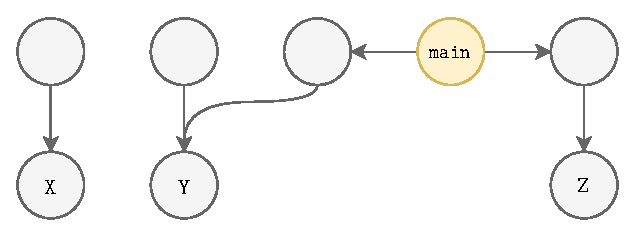
\includegraphics[scale=0.55]{images-paper/callgraph_cases}
    % X, Y, Z = target nodes
% XS, YS, ZS = source nodes
% M = 'main' context node

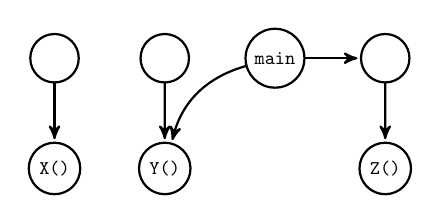
\begin{tikzpicture}[->,>=stealth',shorten >=1pt,auto,node distance=2cm,
                    semithick,thick,scale=0.7, every node/.style={transform
                    shape}] \tikzstyle{every state}=[fill=white,draw=black,text=black]

  \node[state] 	(XS)                    {};
  \node[state]  (YS) [right of = XS]    {};
  \node[state]  (M)  [right of = YS]    {\tt{main}};
  \node[state]  (ZS) [right of = M]     {};
  \node[state]  (X)  [below of = XS] 	{\tt{X()}};
  \node[state]  (Y)  [below of = YS]    {\tt{Y()}};
  \node[state]  (Z)  [below of = ZS]    {\tt{Z()}};

  \path (XS) edge node {} (X)
  		(YS) edge node {} (Y)
  		(M)  edge [bend right] node {} (Y)
  		(M)  edge node {} (ZS)
  		(ZS) edge node {} (Z);
\end{tikzpicture}
    \caption{Callgraph analysis: The bottom nodes represent functions
    containing missed output candidates, the top nodes depict entry points to
    them.}
    \label{fig:callgraph} 
\end{figure}

%Like for include expressions, we again sampled dead function cases and
% identified the lack of direct call sites to those functions. As described in
% Section \ref{sec:inaccessible}, functions despite having no direct call sites
% were called through indirect call features. We identified dynamically
% assembled expressions (function names) to be responsible for failed attempts
% of calling a function indirectly as the resolved function name eventually
% contained symbolic values. These expressions, as well as include expressions,
% contained information dependent on the system environment.

For failed function calls to functions containing not-reached output
candidates we measured how many of those functions were only, or
partially accessibly through indirect function invocation mechanisms (see
Section \ref{sec:experiment_dynamicfeatures}). As Figure
\ref{fig:output_candidate_explanation} illustrates, around 80 percent (except
for \sf{TimeClock}) all missed output candidates of each system were only
accessible through callback candidates, i.e., functions that are only
accessible through indirect calling mechanisms.

\section{Lessons Learned}
In this section we summarize the insights gained from our observations during
the implementation as well as the from the results obtained by our experimental
evaluation.

\paragraph{Dynamic features are problematic.}
From out observations with \sf{WordPress} in Section \ref{sec:3} we learn that
dynamic language features, in particular include expressions and indirect function
invocations, in combination with symbolic values cannot be evaluated accurately
since concrete values are required. For our observations we were able to explain most
of the missed output candidates with indirect function invocations. For include
expressions we are indeed able to resolve most expressions successfully, yet we
do not distinguish between static and dynamic includes in this case study as
this would exceed the scope of our paper. However, we believe it is plausible
to assume that defective include expressions can cause a cascade of missing
files and subsequent includes.
Throughout the experiment we have seen that dynamic features, are prevalent for
modern PHP systems as they serve a genuine purpose in the programming language.
Nevertheless their usage in situations when combined with assumed symbolic
values restricts symbolic execution and any tool leveraging results obtained
from that.

\paragraph{Bypassing conceptual limitations.}
Symbolic execution is used to approximate client page output since it allows to
unfold the staged nature of dynamic web applications. Aside from conceptual
limitations in the systems studied, limitations can be addressed. To use
approaches incorporating symbolic execution with dynamic web applications in
the long run, more concrete input, similar to test oracles, needs
to be provided to decrease the number of assumed symbolic inputs and avoid
dynamic features being confronted with symbolic values. Also, if the usage of
tools using static output approximation with symbolic execution is intended,
avoiding dynamic features that are prone to be inaccurately executed for
symbolic execution  may be an adjustment strategy to program in an analyzable
way. 

\paragraph{Practical tools require practical evaluation.}
Last, we want to address the limited informative value of analyses and tools
presented in previous work
\cite{Nguyen:2011:AFH:2190078.2190142,Nguyen:2014:BCG:2635868.2635928,Nguyen:2015:CPS:2786805.2786872,Nguyen:2015:VIS:2819009.2819140,minamide_static_2005,wassermann2007sound}
where only small PHP systems have been studied. These papers introduce
techniques for static output approximation of PHP web applications
\cite{minamide_static_2005,Nguyen:2014:BCG:2635868.2635928,wang_automating_2012} or propose tools
based on respective approximations
\cite{Nguyen:2011:AFH:2190078.2190142,Nguyen:2014:BCG:2635868.2635928,Nguyen:2015:CPS:2786805.2786872,Nguyen:2015:VIS:2819009.2819140,wassermann2007sound,wassermann_static_2008}.
As these approaches address practical use cases, they require a more and further comprehensive evaluation in order to  better understand possible limitations and assess their practicality, in particular for large-scale systems.

\paragraph{The road so far.}
For this paper, the extension of the symbolic execution \sf{PhpSync} \cite{Nguyen:2014:BCG:2635868.2635928}
support for object-oriented programming was not the main goal, yet necessary to
symbolically execute modern PHP systems. The observations regarding object
target space explosion for method calls documented in Section
\ref{sec:experiment_dynamicfeatures} are only anecdotal and, with the exception
of \sf{WordPress}, we did not notice any significant impact on scalability.
Nevertheless, more research is required to better and systematically understand
possible drawbacks of object-oriented symbolic execution. 
This question though is beyond the scope of this paper, as we aimed
to explore limitations of the practicality and scalability of static output
approximation using symbolic execution. Future work might address design
guidelines to enable programming analyzable applications, tool support to scale
the number of assumed symbolic inputs or systematically provide concrete data
to increase the practical benefit of the tools described above.


\section{Related Work} \label{sec:related_work}

\paragraph{Symbolic Execution}
Symbolic execution \cite{King1976,Darringer1978} remained an conceptual approach
for decades, but has been refined and extended over the last years. Several
approaches incorporating constraint solving and leveraging concrete execution
anlongside symbolic execution emerged and enable automated test case generation
and testing; the scalability of these approaches is still challenged by path
explosion and constraint solving \cite{CadarSen2013}. 

Dynamic symbolic execution \cite{CadarSen2013} incorporates symbolic execution
alongside concrete execution and ahs shown promising results in automated test
generation and testing \cite{artzi_finding_2008,artzi_finding_2010,DynamicWassermann} for PHP web
applications and might help mitigate the conceptual limitations faced with
symbolic values and dynamic features for future work on output-oriented
symbolic execution.

An overview about recent evolution of symbolic execution is provided by work of Cadar et al.
\cite{CadarSen2013}, as well as a more tool-centered perspective \cite{Cadar2011}.

\paragraph{Static Output Approximation}
To approximate program slices for web
applications, Ricca et al. \cite{tonella_web_2005,tonella_2001,tonella_2002} approximate
dynamically generated output. For output generating statements, such as \tt{echo} or
\tt{print}, all strings are unquoted (code extrusion). If those statements
contain variables, these are linked to string concatenations using a
proposed flow analysis called \emph{string-cat propagation}. From these
flows representing approximated output subsequent program slices are computed.

Minamide \cite{minamide_static_2005} approximates client page output
of web applications by describing possible output by a context-free
grammar that is constructed statically from the PHP code for a given regular
expression of user input. The constructed grammar enables analyses such as
detecting cross-site scripting vulnerabilities by checking whether user input
has been sanitized, and HTML validation by determining whether the constructed
grammar is contained in a depth-bound HTML grammar. Based on Minamide's
approximation approach several vulnerability analyses addressing cross-site
scripting \cite{wassermann_static_2008} and SQL injection
\cite{wassermann2007sound} have been proposed. Wang et al.
\cite{wang_locating_2010} utilizes this string analysis to detect strings
visible at the browser and enable internationalization of web applications.
    
Another approach is proposed by Wang et al. \cite{wang_automating_2012}, where
output for a web application is approximated using a hybrid approach: A
dynamic webpage is executed with concrete input and the execution is
recorded at runtime. Changes in the client-side output then can be mapped to 
corresponding PHP code using static impact analysis.

\paragraph{Dynamic Features}
According to a case study by Hills et al. \cite{Hills:2013:ESP:2483760.2483786}
of the feature usage in PHP, based on a corpus of state-of-the-art-projects,
dynamic includes are less frequently used than static includes, but usage
frequency is varying from system to system. Further work by Hills et al.
\cite{hills2014static,hills2014php} approaches static resolution of dynamic includes using
both context-insensitive resolution on file level by simplifying PHP constants; and context-sensitive on program level for transitive includes. In spite of
promising results, these approaches, similar to our results, face limitations
for truly dynamic includes if resolution is not sound due to information not
being available in the source code like database query results. 

\section{Conclusion}
In this paper we have addressed symbolic execution of PHP web applications that
is used for client page output approximation. This approximations are leveraged
be several developer tools for PHP, yet have not been evaluated for larger
systems. We re-implemented and extended an existing symbolic execution engine
to analyze several real-world PHP applications with the intention to evaluate
the scalability of symbolic execution for PHP. Our work illustrates the
necessity of more comprehensive evaluation of developer tools as
previous work did not explore these limitations. Dynamic features of PHP in
combination with symbolic values though hinder precise symbolic execution and
limit the scalability and practicality of tools on symbolically approximated
client page output.

In the future we would like to use dynamic symbolic execution for output
approxiamtion and possibly bypass existing limitations, as dynamic symbolic
execution has shown to be promising for automated testing and verification.

%\newpage
%References
\bibliographystyle{ACM-Reference-Format}
\bibliography{bibliography} 

\end{document}
